\documentclass{CUP-JNL-DTM}%


%%%% Packages
\usepackage{graphicx}
\usepackage{multicol,multirow}
\usepackage{amsmath,amssymb,amsfonts}
\usepackage{mathrsfs}
\usepackage{amsthm}
\usepackage{rotating}
\usepackage{appendix}
% For JDM please remove the natbib package:
\usepackage[numbers]{natbib}
% And use biblatex-apa with a .bib file to format your references according to the APA7 style.
% \usepackage[natbib,style=apa]{biblatex}
% \addbibresource{your-refs.bib}
\usepackage{ifpdf}
\usepackage[T1]{fontenc}
\usepackage{newtxtext}
\usepackage{newtxmath}
\usepackage{textcomp}
\usepackage{xcolor}
\usepackage{lipsum}
\usepackage{float}
\usepackage{subcaption}
\usepackage[colorlinks,allcolors=blue]{hyperref}


\newtheorem{theorem}{Theorem}[section]
\newtheorem{lemma}[theorem]{Lemma}
\theoremstyle{definition}
\newtheorem{remark}[theorem]{Remark}
\newtheorem{example}[theorem]{Example}
\numberwithin{equation}{section}


\jname{Universidad San Francisco de Quito}
\articletype{}
\artid{}
\jyear{2025}
\jvol{}
\jissue{}
%\raggedbottom


\begin{document}

\begin{Frontmatter}

\title[Article Title]{High Energy physics project}

% There is no need to include ORCID IDs in your .pdf; this information is captured by the submission portal when a manuscript is submitted. 
\author[1]{Jos\'e David Ochoa Flores}

\authormark{Author Name1 \textit{et al}.}

\address[1]{\orgdiv{Maestr\'ia de F\'isica}, \orgname{Universidad San Francisco de Quito}, \orgaddress{\city{Quito}, \country{Ecuador}}}


\authormark{Jos\'e Ochoa}

\keywords{Simulation, chain, Drell-Yan, Beyond Standard Model, FeynRules}

\abstract{he following project aims to simulate a BSM model using the \textit{FeynRules} package. For this, we first start by doing the full simulation chain of a Drell-Yan process including the generation of events, the simulation of the detector, and the invariant mass distribution of the electrons and muons simulated. We include other example intermediate chains of simulation and show the difficulties encountered.}

\end{Frontmatter}

% Some math journals (FLO) require a table of contents. Comment out this line if no ToC is needed.
%\localtableofcontents

\section[Seccion 1]{Introduction}
The use of simulations in high energy physics is an incredible useful tool to understand the physics of the processes that we are studying. Several tools have been developed and are useful for this purpose. Among the most important tools are \textit{FeynRules}, \textit{MadGraph}, \textit{Pythia} and CMSSW. 

\section{DY}{Drell-Yan process}


The simplest chain in feynrules -> UFO -> Madgraph (Pythia) -> LHE -> CMSSW -> python (uproot)



\begin{figure}[H]
    \begin{subfigure}{.5\textwidth}
      \centering
      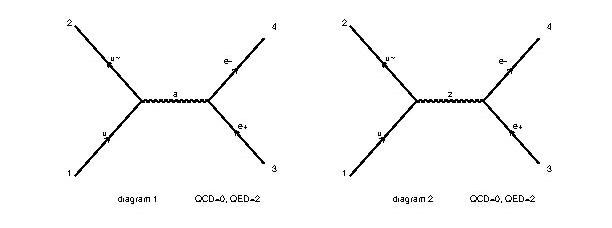
\includegraphics[width=1.1\linewidth]{img/dy_sm_diagrams.jpg}
      \label{fig:sm_dy1}
    \end{subfigure}%
    \begin{subfigure}{.5\textwidth}
      \centering
      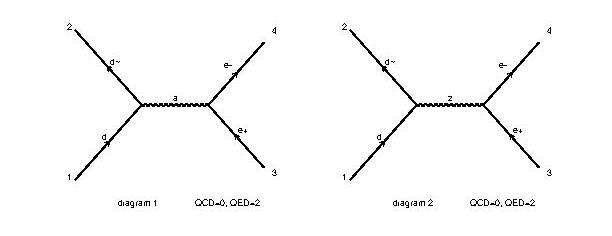
\includegraphics[width=1.1\linewidth]{img/dy2_sm_diagrams.jpg}
      \label{fig:sm_dy2}
    \end{subfigure}
    \caption{SM DY feynman diagrams}
    \label{fig:sm_dy}
\end{figure}



\begin{figure}[H]
    \begin{subfigure}{.5\textwidth}
      \centering
      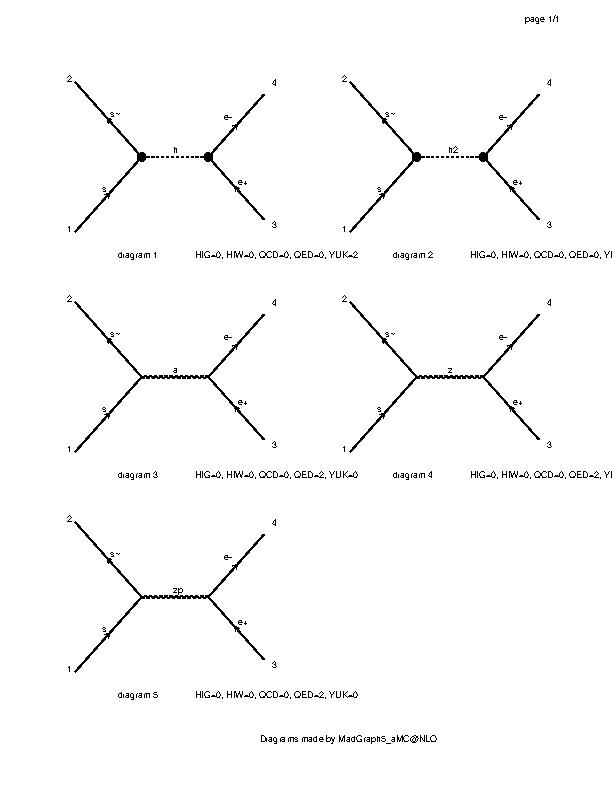
\includegraphics[width=1\linewidth]{img/dy_bsm_diag.jpg}
      \label{fig:bsm_dy1}
    \end{subfigure}%
    \begin{subfigure}{.5\textwidth}
      \centering
      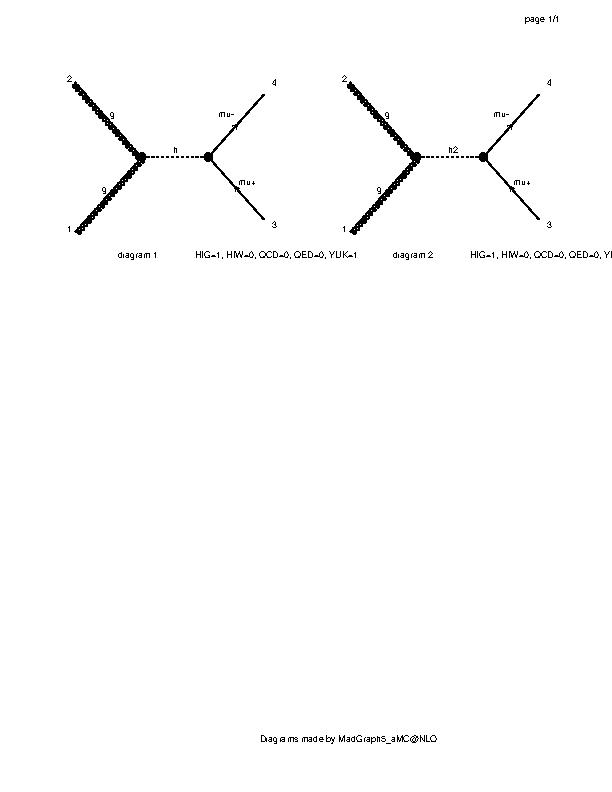
\includegraphics[width=1\linewidth]{img/bsm_dy_diag2.jpg}
      \label{fig:bsm_dy2}
    \end{subfigure}
    \caption{BSM DY feynman diagrams}
    \label{fig:bsm_dy}
\end{figure}


\begin{figure}[H]
    \begin{subfigure}{.5\textwidth}
      \centering
      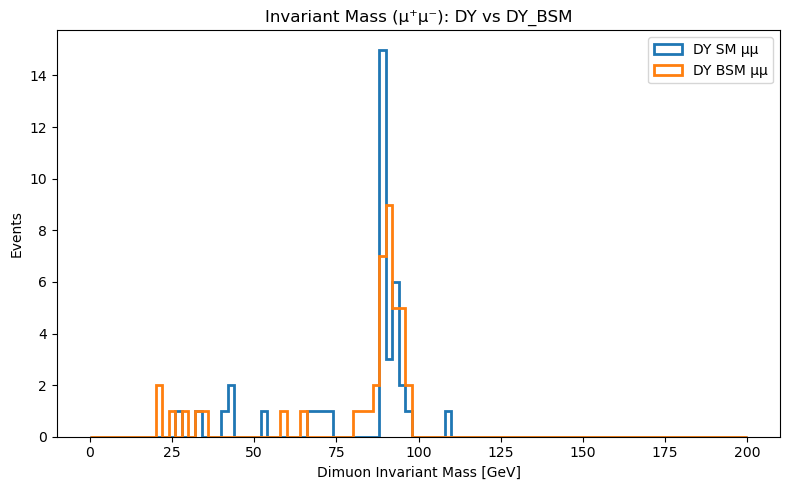
\includegraphics[width=.85\linewidth]{img/mumu_comp.png}
      \caption{Dimuon invariant mass}
      \label{fig:mumu}
    \end{subfigure}%
    \begin{subfigure}{.5\textwidth}
      \centering
      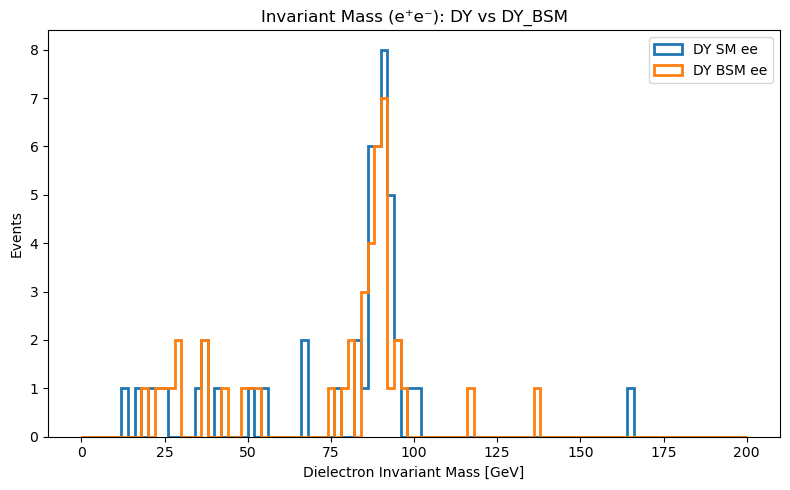
\includegraphics[width=.85\linewidth]{img/ee_comp.png}
      \caption{Dielectron invariant mass}
      \label{fig:ee}
    \end{subfigure}
    \caption{Dilepton invariant mass comparison for SM DY and BSM DY} 
    \label{fig:imass}
\end{figure}



\begin{figure}[H]
    \begin{subfigure}{.5\textwidth}
      \centering
      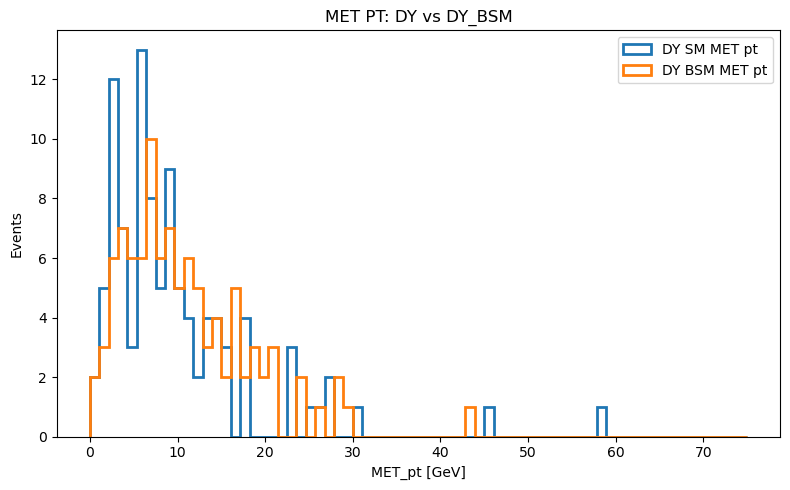
\includegraphics[width=.85\linewidth]{img/met_pt.png}
      \caption{MET pt}
      \label{fig:sm_metpt}
    \end{subfigure}%
    \begin{subfigure}{.5\textwidth}
      \centering
      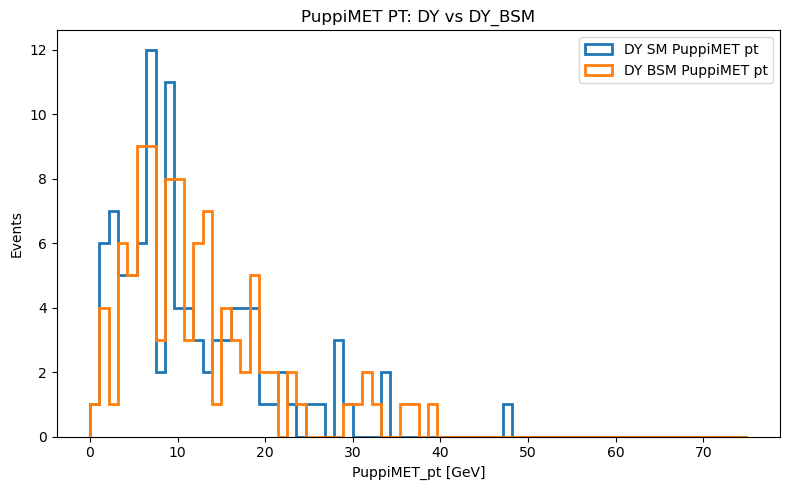
\includegraphics[width=.85\linewidth]{img/pmet_pt.png}
      \caption{PuppiMET pt}
      \label{fig:sm_pmetpt}
    \end{subfigure}
    \caption{MET pt and PuppiMET pt comparison for SM DY and BSM DY}
    \label{fig:metpt}
\end{figure}

\begin{figure}[H]
    \begin{subfigure}{.5\textwidth}
      \centering
      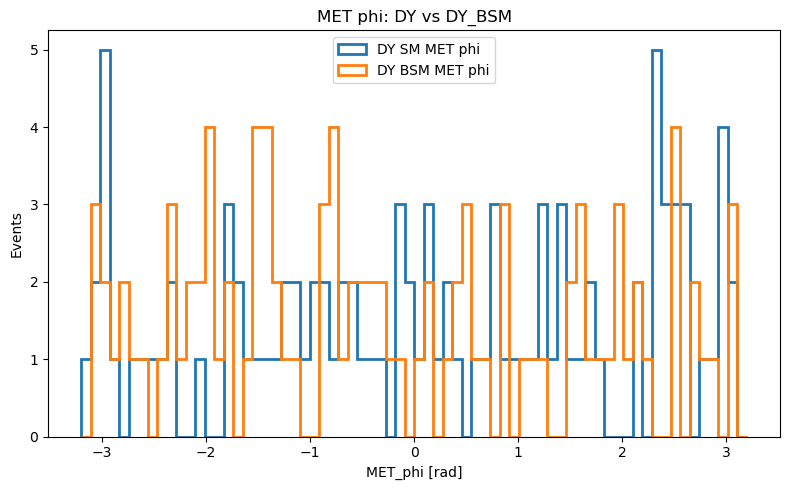
\includegraphics[width=.85\linewidth]{img/met_phi.png}
      \caption{MET phi}
      \label{fig:sm_metphi}
    \end{subfigure}%
    \begin{subfigure}{.5\textwidth}
      \centering
      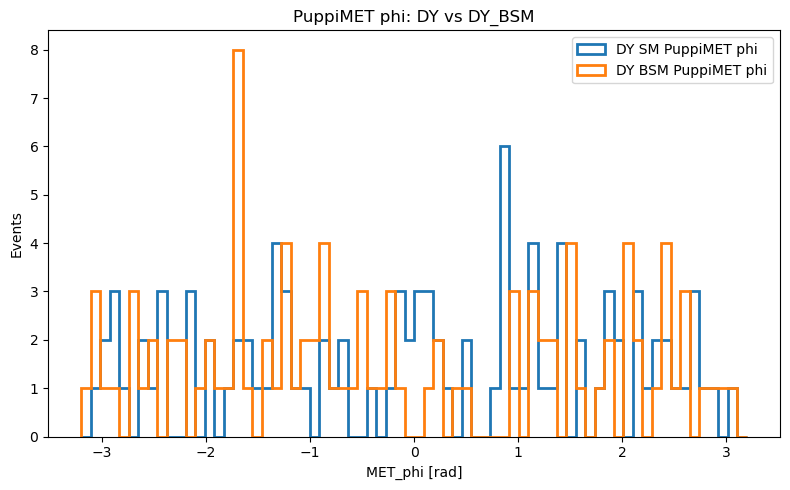
\includegraphics[width=.85\linewidth]{img/pmet_phi.png}
      \caption{PuppiMET phi}
      \label{fig:sm_pmetphi}
    \end{subfigure}
    \caption{MET phi and PuppiMET phi comparison for SM DY and BSM DY}
    \label{fig:metphi}
\end{figure}

\section{Conclusion}


\begin{Backmatter}
% For JDM please remove this \begin{thebibliography}...\end{thebibliography} list.
% Use biblatex-apa (see instructions in preamble) instead, and write \printbibliography here to print the reference list in APA7 style.
\begin{thebibliography}{}


% Exotic Decays of the 125 GeV Higgs Boson" by Curtin, Essig, Gori, Jaiswal, Katz, Liu, Liu, McKeen, Shelton, Strassler, Surujon, Tweedie and Zhong. (​arXiv:1312.4992) "Illuminating Dark Photons with High-Energy Colliders", by Curtin, Essig, Gori, Shelton (​arXiv:1412.0018)


\end{thebibliography}   

\end{Backmatter}

\end{document}
